\section{Introduction}

The useful next step in a reasoning trace depends on what the solver can do after taking it. A legally executed arithmetic move can be a detour for a solver that lacks a shortcut, then become useful once the solver gains it. Process advantage verifiers make that distinction by measuring progress against a specified continuation policy~\citep{setlur2024rewarding}. Step validity answers a different question: whether the move followed the task rules at all. If a verifier keeps both labels for future use, a solver release can make one field stale while leaving the other correct.

This suggests attaching different expiration conditions to the two fields. Keep a checked validity label while the grammar is unchanged, and refresh the progress label only when the new release may change a continuation it depends on. The semantic distinction is straightforward. The computational claim is not: a release can touch many continuation neighborhoods without changing their answers, and a recomputation baseline can share work across labels. To justify a row-level guard, selective refresh must beat both invalidating the whole guarded row and simply recomputing the solver-dependent part from a shared cache.

We test this claim in a bounded arithmetic task where legality is fixed, progress is exact, and the only change is a new continuation move. The guard has no false negatives for a release of this form. We compare three refresh policies at fixed operation caps against both a stale store and an independent oracle. A second release reverses the direction of the new move and increases how many labels change, without altering the task grammar.

The guard recovers stale labels, but its benefit does not clear the preregistered bar. On release A at the primary cap, split labels reach 96.53\% versus 96.51\% for whole-label refresh and 96.89\% for memoized recomputation (\cref{tab:primary}). The latter spends its budget on continuation attempts rather than screening rows. At a larger cap all three refresh policies reach exact labels on release A, while memoized recomputation spends fewer operations (\cref{fig:cap,sec:diagnostic}). This is a failure of the tested refresh primitive, not a reason to confuse validity with progress.

\begin{figure}[t]
\centering
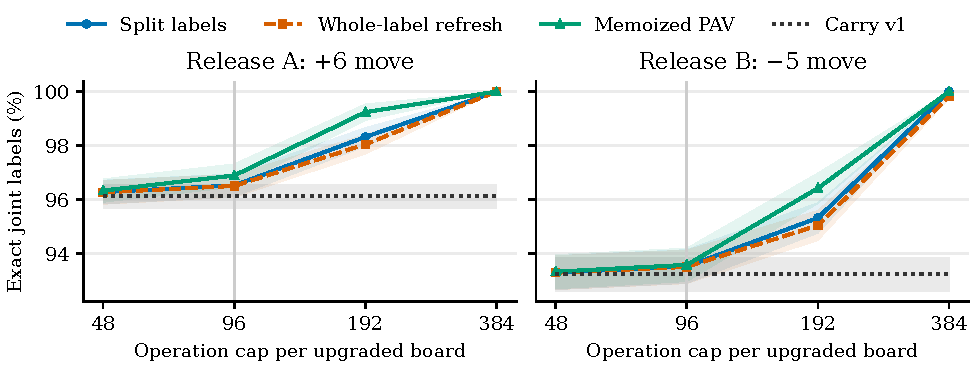
\includegraphics[width=\linewidth]{accuracy.pdf}
\caption{\textbf{Memoized recomputation is at least as accurate as guarded split refresh at every tested cap.}
Exact joint-label accuracy on upgraded arithmetic boards, averaged over 32 paired streams; bands show marginal 95\% stream-level intervals, not intervals for contrasts. The dotted horizontal line leaves labels at v1; the vertical marker indicates the primary cap, 96 operations per upgraded board. The right panel is the descriptive second release.}
\label{fig:cap}
\end{figure}
